\documentclass[a4paper,11.5pt]{article} % тип документа


%%%Библиотеки
%\usepackage[warn]{mathtext}	
%\usepackage[T2A]{fontenc} % кодировка
\usepackage[utf8]{inputenc} % кодировка исходного текста
\usepackage[english,russian]{babel} % локализация и переносы
\usepackage{caption}
\usepackage{listings}
\usepackage{amsmath,amsfonts,amssymb,amsthm,mathtools}
\usepackage{wasysym}
\usepackage{graphicx}%Вставка картинок правильная
\usepackage{float}%"Плавающие" картинки
\usepackage{wrapfig}%Обтекание фигур (таблиц, картинок и прочего)
\usepackage{fancyhdr} %загрузим пакет
\usepackage{lscape}
\usepackage{xcolor}
\usepackage[normalem]{ulem}
\usepackage{hyperref}

\usepackage{mathtext}
\newcommand{\angstrom}{\text{\normalfont\AA}}
%%%Конец библиотек


%%%Настройка ссылок
\hypersetup
{
	colorlinks=true,
	linkcolor=blue,
	filecolor=magenta,
	urlcolor=blue
}
%%%Конец настройки ссылок


%%%Настройка колонтитулы
\pagestyle{fancy}
\fancyhead{}
\fancyhead[L]{Лабораторная работа 1}
\fancyhead[R]{Курневич Станислав, группа Б01-008а}
\fancyfoot[C]{\thepage}
%%%конец настройки колонтитулы



\begin{document}
	%%%%Начало документа%%%%
	
	%%%Начало титульника
	
	\begin{titlepage}
		
		\newpage
		\begin{center}
			\normalsize Московский физико-технический институт \\(госудраственный 			университет)
		\end{center}
		
		\vspace{6em}
		
		\begin{center}
			\Large Лабораторная работа по вычислительной математике\\
		\end{center}
		
		\vspace{1em}
		
		\begin{center}
			\large \textbf{Лабораторная работа 2}
		\end{center}
		
		\vspace{2em}
		
		\begin{center}
			\large Работу выполнил:\\	
			Курневич Станислав Витальевич\\
			Группа Б01-008а
		\end{center}
		
		\vspace{\fill}
		
		\begin{center}
			Долгопрудный \\10.10.2022
		\end{center}
		
	\end{titlepage}
	%%%Конец Титульника
	
	%%%%%%Начало работы с текстом%%%%%%
	
    \section{Постановка задачи}
    В лабораторной работе предлагается решить уравнение: $Ax = f$ двумя методами: прямым методом и итерационным методом. Так же нужно определить невязку каждого метода, найти $\lambda_{min}, \lambda_{max}$, определить число обусловленности матрицы.

    \section{Выполнение}
    Выбрал матрицу $A$ для выполнения работы под номером б).
    \begin{figure}[H]
		\center{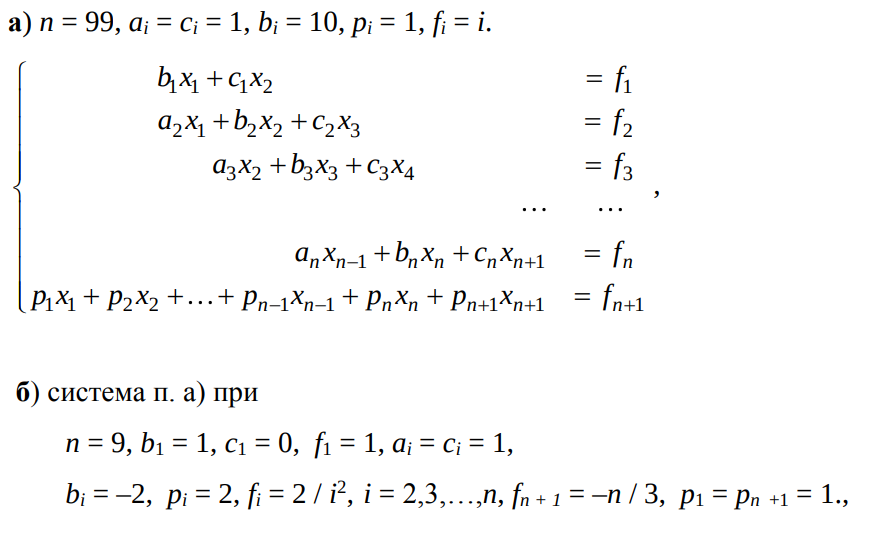
\includegraphics[scale = 0.4]{images/matrix.png}}
	\end{figure}
    Для начала определил число обусловленности матрицы $\mu$ для трех норм.
    \begin{figure}[H]
		\center{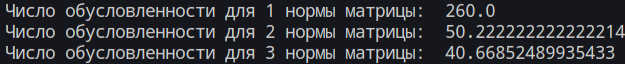
\includegraphics[scale = 0.4]{images/mu.png}}
	\end{figure}
    Далее буду использовать 3 норму, для которой число обусловленности равно $\mu = 40.6685$.
    \\
    С помощью степенного метода нашел $\lambda_{max}$ и $\lambda_{min}$:
    \begin{figure}[H]
		\center{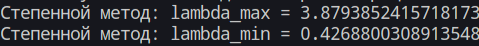
\includegraphics[scale = 0.4]{images/lambda.png}}
	\end{figure}

    \subsection{Прямой метод}
    Проверил главные миноры матрицы $A$, они оказались не нулевыми $\Rightarrow$ можно применить метод $LU-$разложения.
    Невязка получилась равной $\approx 9 \cdot 10^{-16}$
    
    \subsection{Прямой метод}
    Невязка получилась равной $\approx 9 \cdot 10^{-7}$

    \end{document}